\begin{figure}[]
  \centering
  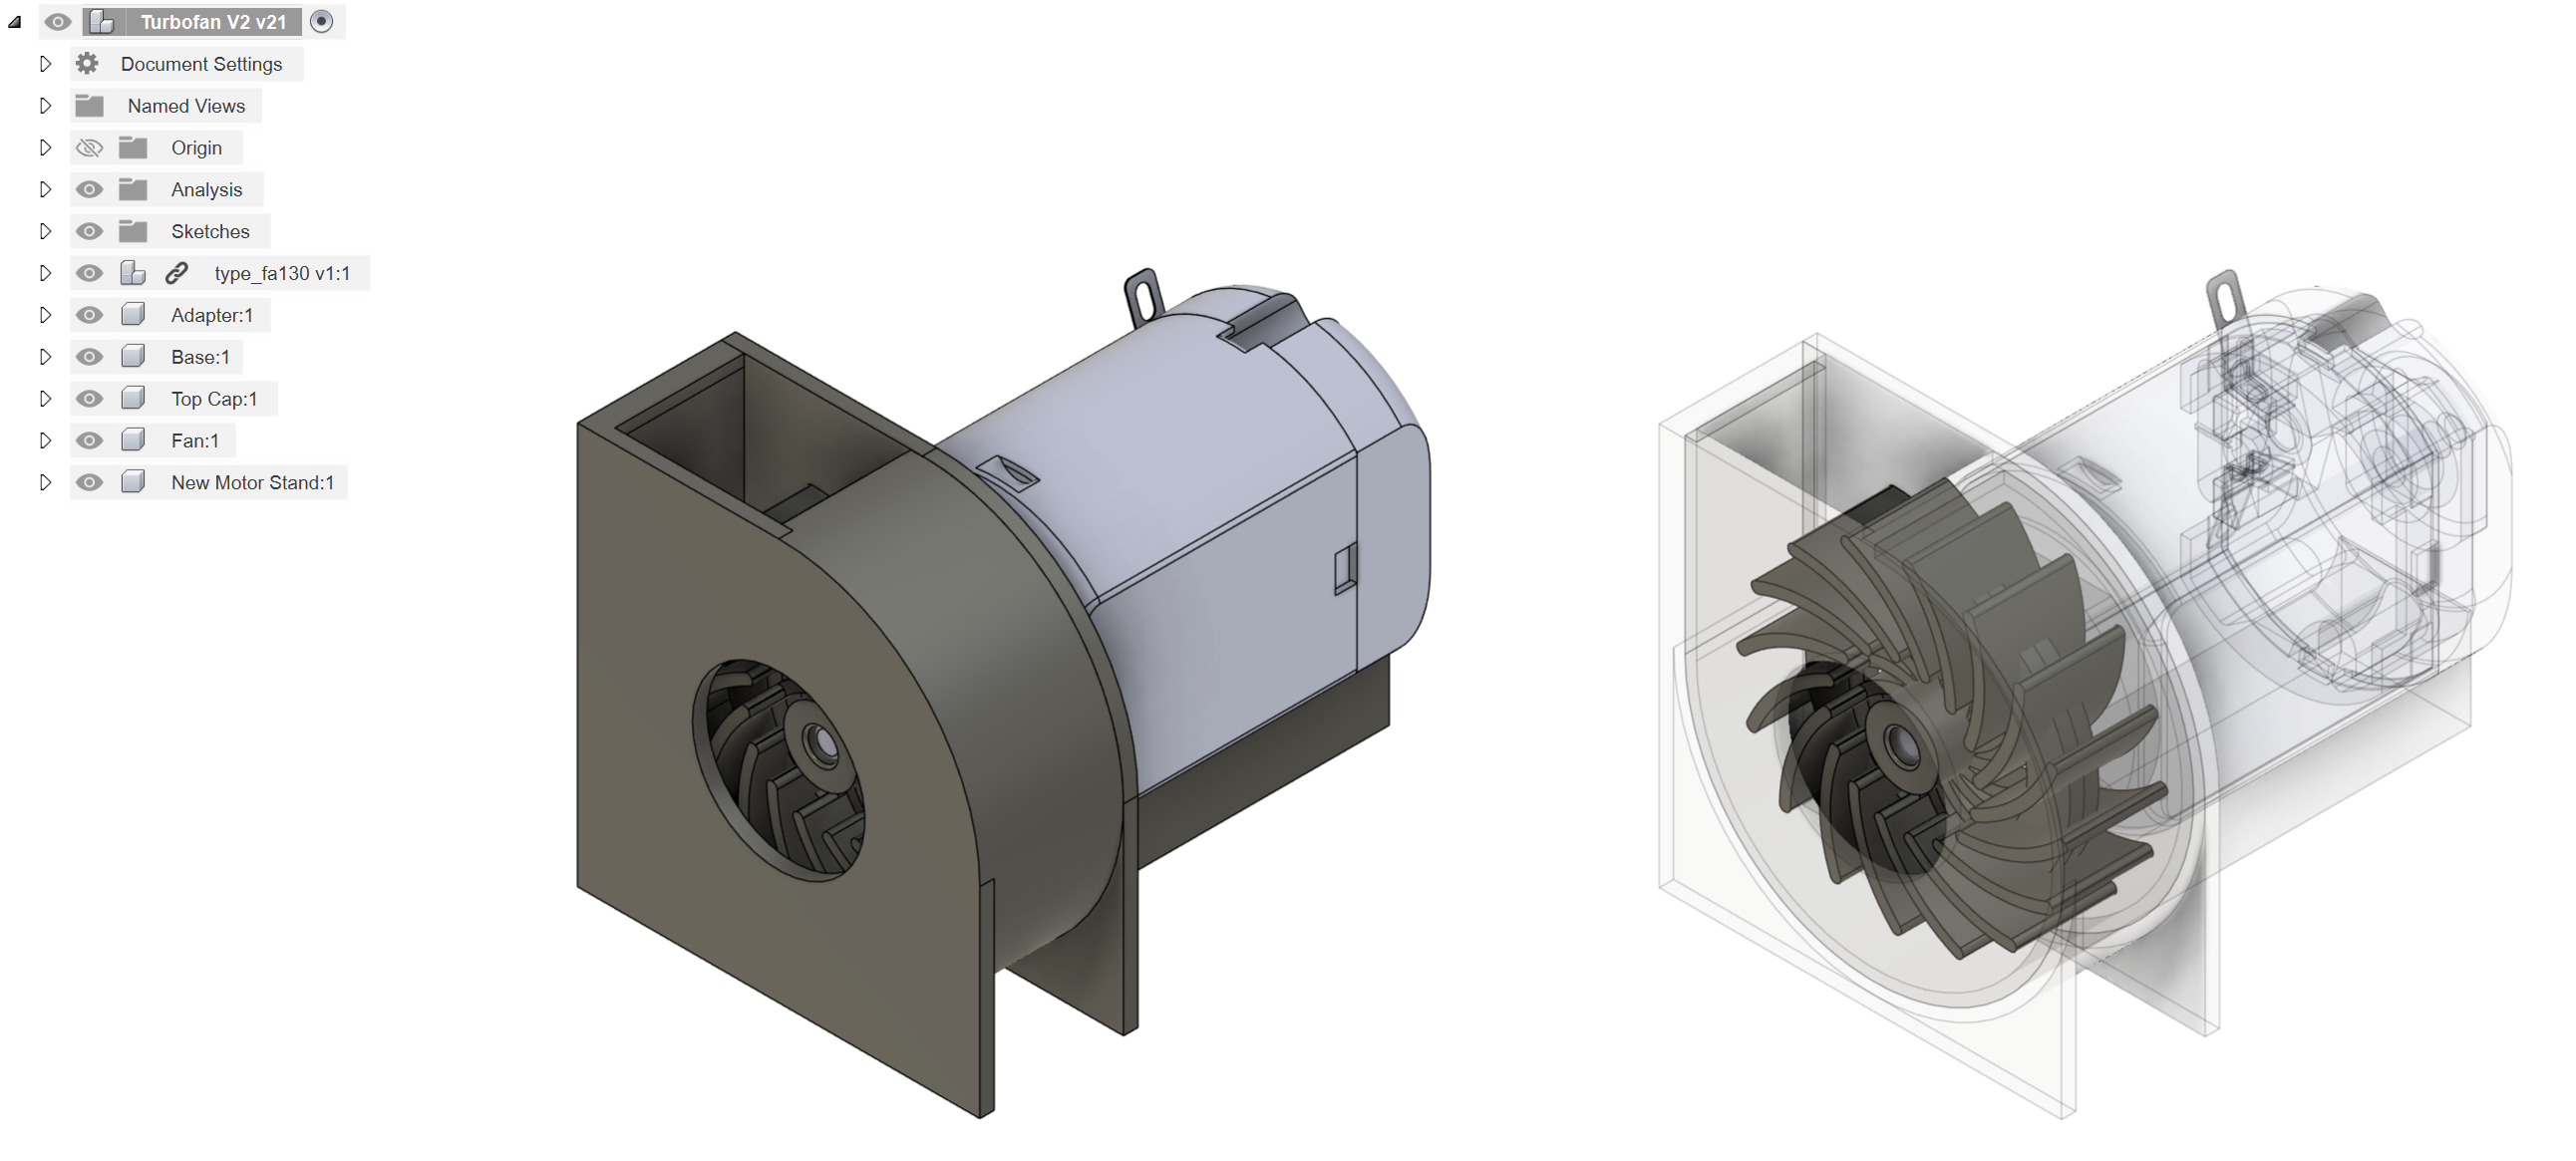
\includegraphics[width=\linewidth]{Images/Slice 2.png}
  \caption{The turbofan model}
  \label{fig:fan}
  \Description{}
\end{figure}


At the beginning of this phase, we had already known what we aimed to create, so the initial period was planning the necessary hardware. As we were ready to implement a high-fidelity model, our requirements had been refined down to the specific components needed to fulfill certain functions. The functionalities we hoped to implement include:

\begin{enumerate}
    \item Users can know the lighting conditions of the other person's environment by observing the LED strip on the top of the device.
    \item Users can press and hold a button to record an audio message, and release the button to send this message.
    \item An red LED indicator lights up when a message is received.
    \item An yellow LED indicator lights up when the other person's location has a sunny weather.
    \item An blue LED indicator lights up when the other person's location is raining or snowing
    \item Users can play the received voice message by rotating the top of the snow globe.
    \item The device's top platform starts rotating when playing a voice message.
    \item Users can send a snowstorm signal to the other person by shaking the device.
\end{enumerate}

I began work on the high-fidelity prototype by exploring the creation of a high-fidelity snow globe shell, which first led me to learn about glass blowing since we expect the glass lab could help us create the shells. Specifically, I delved into its limitations of glass blowing technology and briefly designed the appearance of the snow globe. Following this, I produced a draft print to showcase our design to a lab member for consultation, assessing whether our draft or blueprint met their capabilities. However, we were informed that they could not assist in making the globe but could help us cut specific products to meet our requirements, potentially orderable through the university's system. Consequently, we opted for a 500 mL rounded flask that matched our needs. Then we were told ordering the chemical equipment for our project cannot be achieved and we were recommended to use the SLA printer or the vacuum former in the Lili's prototype lab to construct our product.

Thus, I started learning how SLA printers operate and their application. SLA printers, in theory, could produce highly transparent objects, aligning with our requirements for the next phase. Upon visiting the lab to inspect the SLA equipment, we were shown a component printed by the machine, which was the most transparent option available, albeit still too opaque for our needs. Exploring alternative methods, we learned how to use a vacuum former to create a shell. However, the materials available were insufficient and too prone to deformation, unsuitable for our product, which features a user-interactable snow globe that can be turned to access voice messages. Although using multiple layers of material with a vacuum former could construct a globe, it would significantly reduce the product's transparency. After deliberation, we decided to purchase an existing transparent vessel. While this meant not creating the snow globe ourselves, it was deemed a necessary compromise to maintain project momentum. 
Now when I wrote this text, my reflection is that we should have decided quicker to save the precious time for building other parts or revise our design to something else that is well available.

Nevertheless, I also spent these two weeks learning about Fusion 360.
To evaluate my learning outcomes, I used Fusion 360 to design a turbo fan (see figure \ref{fig:fan}), adapting it to a motor to generate the storm effect inside the snow globe. I found a picture of a laptop turbo fan online for reference and modeled the turbofan using Fusion 360. After three iterations, the design proved highly functional, capable of blowing lightweight materials to simulate snow. And I modeled the fan in a flexible way which benefit a lot when I need to minimize the fan due to size limitataion. This process greatly enhanced my familiarity with Fusion 360. Next, I began designing a double-layer turnable platform, with one layer motor-driven and the other user-operated to turn in only one direction. Discussing the feasibility with Yu, our prototyper, we eventually devised a solution, leading me to model the gears and other structures. I first printed a single-layer platform that could be motor-turned, including the stand for two motors, while considering the design's extendibility. The next step was to create the second layer of ratchet mechanism. However, due to the time limitation I ask help from Yu and he reconstruct the structure from scratch in the way he prefer. 
My role then in the turning mechanism was to establish a proper interface for mounting the structure and to assist with testing upon updates.

\begin{figure}[]
  \centering
  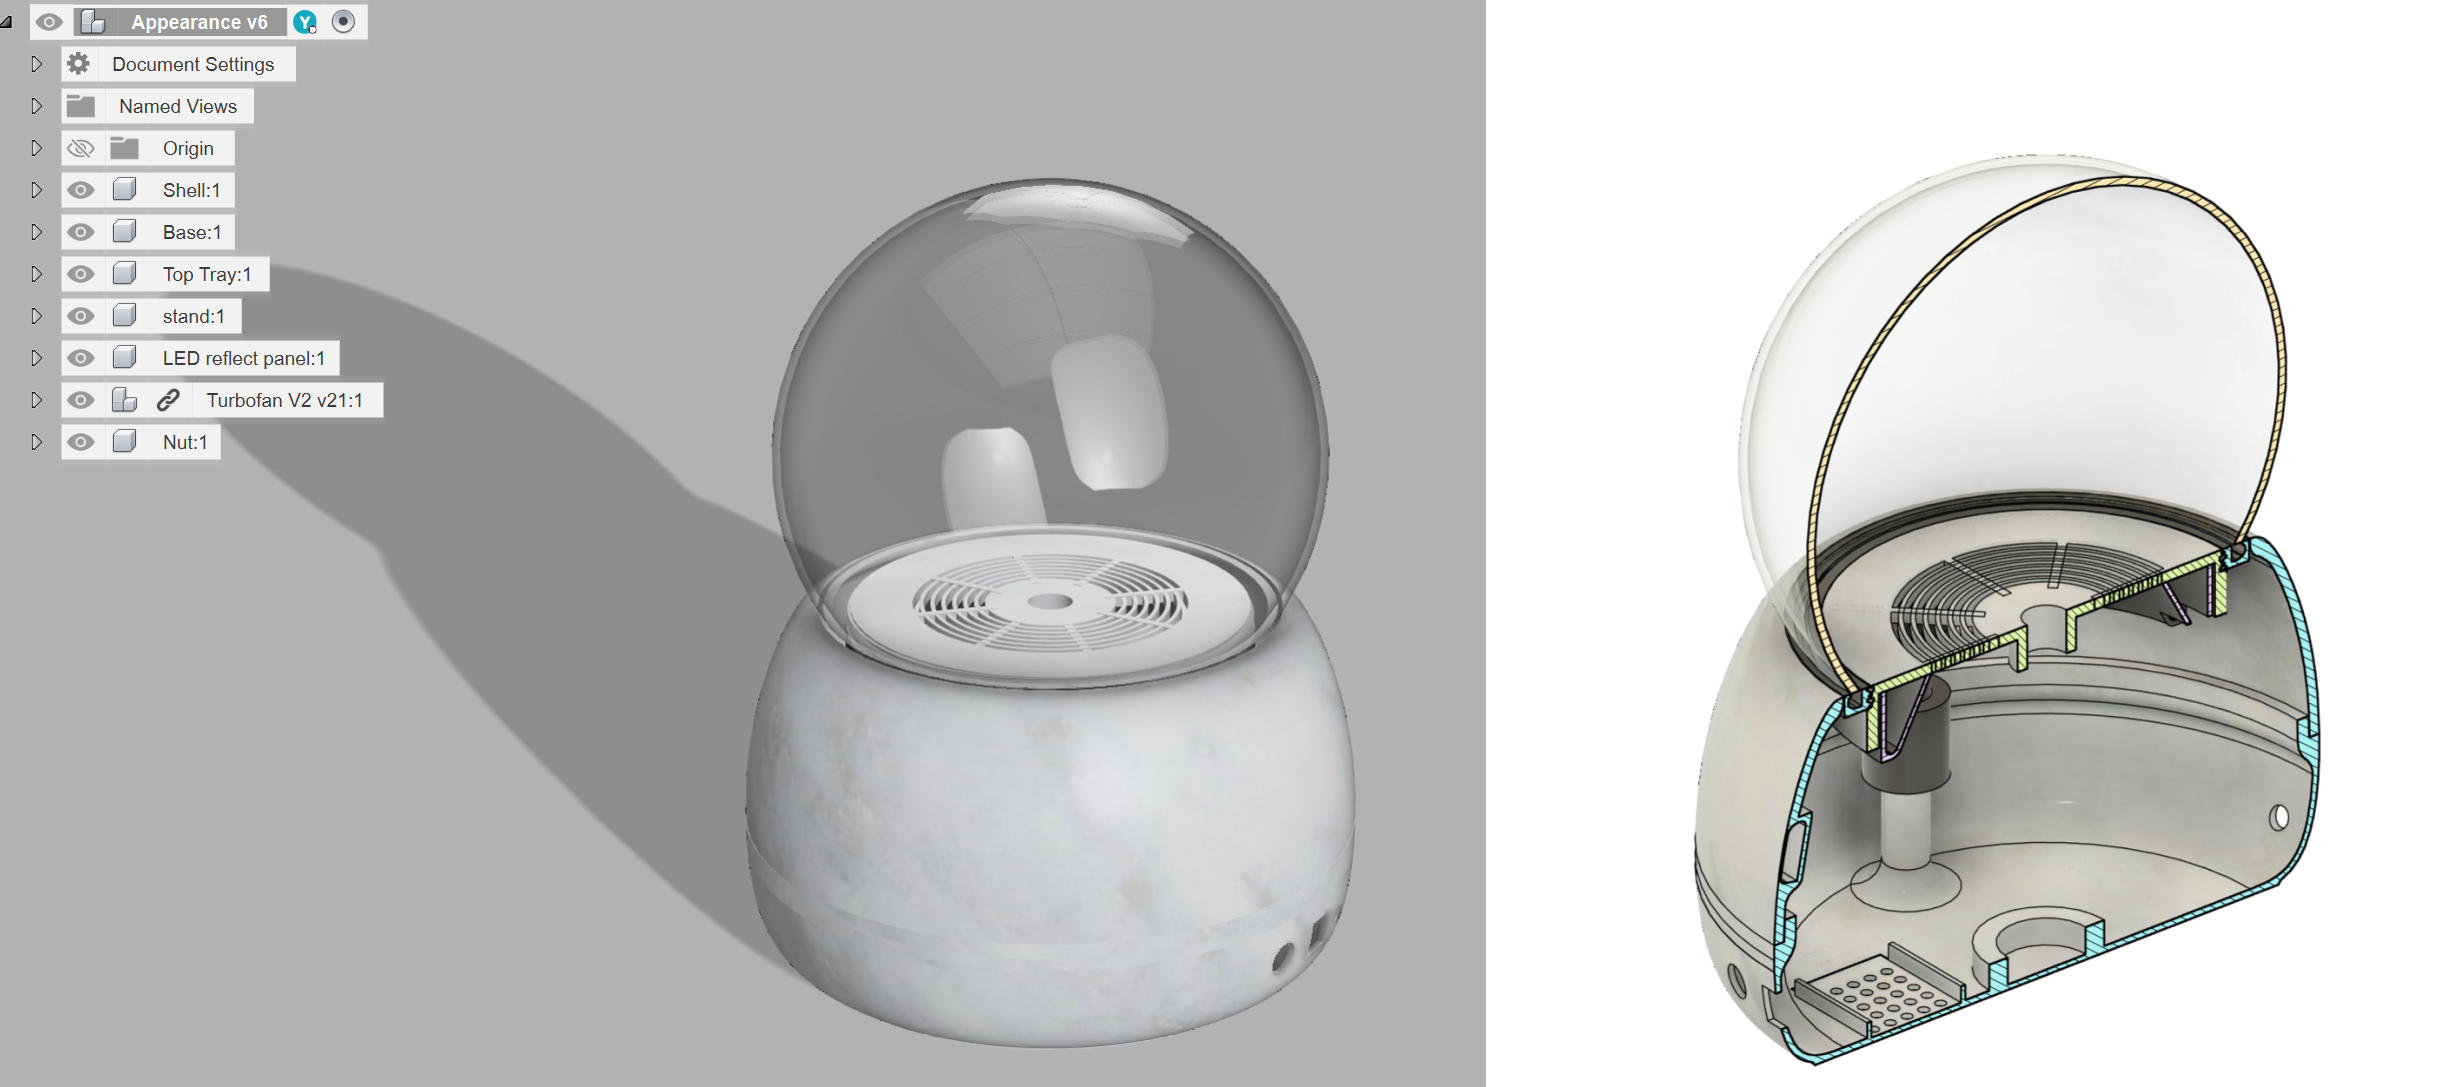
\includegraphics[width=\linewidth]{Images/Slice 3.png}
  \caption{The snow globe appearance design}
  \label{fig:design}
  \Description{}
\end{figure}

I then proceeded to model the base of the snow globe (see figure \ref{fig:design}). My goal was to minimize the base as much as possible, as users will ultimately hold and shake the snow globe in their hands. A snow globe that is unwieldy to pick up with one hand would hinder the user's ability to interact with it. However, this required repeated adjustments and test prints, so I spent a considerable amount of time printing over and over again at this stage. In the final phase of compiling this document, I reflected that I should have initially opted for a solution with a lower margin for error. In summary, after repeated testing and adjustments, I achieved a relatively compact design. After planning the placement of the components, I began the actual printing of the devices we needed. The next step was to assemble all the parts, which took much more time than I had anticipated.
New challenges continually arose, such as our inability to obtain female-to-female wires from the lab, leading us to spend a significant amount of time soldering over forty to fifty wires individually. This also made troubleshooting and modifications difficult. During the assembly phase, we discovered that one microphone module was not functioning properly, and a speaker was damaged. Nonetheless, we adjusted our plans and worked diligently to complete a prototype suitable for presentation. As of the submission of this document, we are still in the process of making it, uncertain of the final outcome (see figure \ref{fig:progress}). However, I hope that by the time you read this, you have already seen our finished product and enjoyed it!


\begin{figure}[]
  \centering
  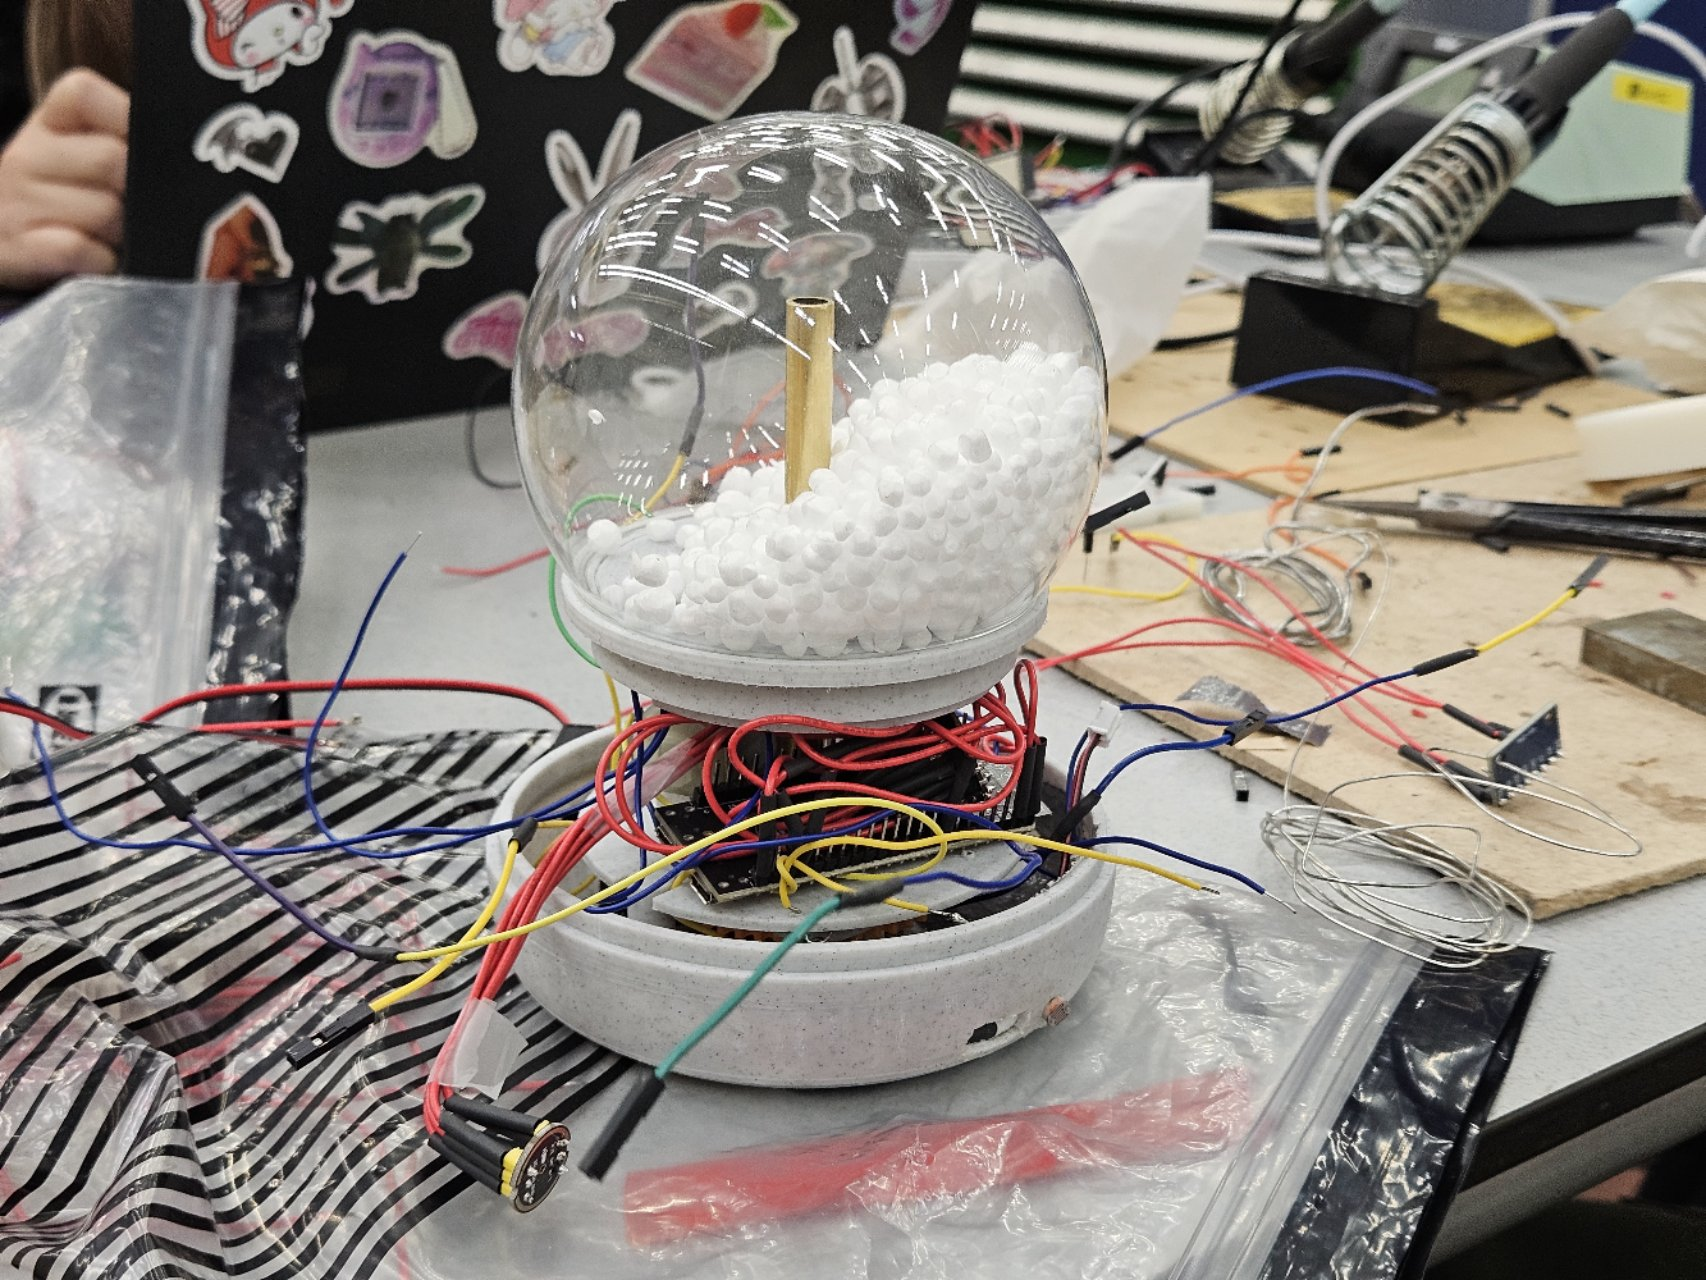
\includegraphics[width=\linewidth]{Images/Progress.jpg}
  \caption{The day when this document is submited}
  \label{fig:progress}
  \Description{}
\end{figure}
